\chaptercustom{3}{THIẾT KẾ HỆ THỐNG VÀ PHÂN TÍCH GIAO THỨC}
\setcounter{section}{3}
\setcounter{equation}{0}
Chương này mô tả topo mạng dựng trên Mininet, giao thức ứng dụng FLSync do nhóm định nghĩa, trình tự thông điệp trong một vòng đồng bộ, và đường đi của dữ liệu qua bốn tầng application, transport, network, link. Cuối chương là kế hoạch bắt gói để lấy bằng chứng thực tế cho các phân tích.

\subsection{Topo mạng}
Hình~\ref{fig:topo} là topo dùng cho mọi kịch bản. Sáu Edge Node \texttt{h1}--\texttt{h6} nối vào Edge Switch \texttt{s1} trong mạng biên 10.0.1.0/24. Edge Aggregator \texttt{agg} nằm cùng mạng này. Để ra khỏi vùng biên, gói phải đi qua Edge Gateway \texttt{r1}: một host Linux bật chuyển tiếp IP, vừa là router giữa hai mạng, vừa là firewall (iptables). Phía bên kia liên kết WAN là mạng cloud 10.0.2.0/24 gồm switch \texttt{s2} và Cloud Server \texttt{cloud}. Số Edge Node tham gia một lần đo ($N$ = 2..6) được chọn bằng tham số dòng lệnh; các host không tham gia vẫn có mặt nhưng không phát lưu lượng.

\begin{figure}[H]
    \centering
    \begin{tikzpicture}[
        host/.style={draw, rounded corners, minimum width=1.1cm, minimum height=0.7cm, font=\small, fill=blue!8},
        sw/.style={draw, minimum width=1.1cm, minimum height=0.8cm, font=\small, fill=gray!15},
        rt/.style={draw, circle, minimum size=1.1cm, font=\small, fill=red!12},
        srv/.style={draw, rounded corners, minimum width=1.9cm, minimum height=0.9cm, font=\small, fill=orange!15, align=center},
    ]
        \foreach \i in {1,...,6} {
            \node[host] (h\i) at (0, {3.25 - (\i-1)*1.3}) {h\i};
        }
        \node[sw] (s1) at (3.2, 0) {s1};
        \foreach \i in {1,...,6} {
            \draw (h\i.east) -- (s1.west);
        }
        \node[font=\scriptsize, align=center] at (1.5, -4.2) {100 Mbps, 1 ms\\(mỗi link truy nhập)\\10.0.1.1--10.0.1.6};
        \node[srv] (agg) at (6.4, 2.4) {Edge Aggregator\\\texttt{agg} 10.0.1.100};
        \node[rt] (r1) at (6.0, -1.6) {r1};
        \node[font=\scriptsize, align=center, below=1pt of r1] {Edge Gateway\\router + firewall\\.1.254 \;|\; .2.254};
        \node[sw] (s2) at (9.9, -1.6) {s2};
        \node[srv] (cloud) at (12.8, -1.6) {Cloud Server\\\texttt{cloud} 10.0.2.200};
        \draw[very thick] (s1) -- node[font=\scriptsize, sloped, above, pos=0.45] {100 Mbps, 1 ms} (agg);
        \draw (s1) -- node[font=\scriptsize, sloped, below, pos=0.5] {100 Mbps} (r1);
        \draw[very thick, dashed] (r1) -- node[font=\scriptsize, above] {WAN, 20 ms} node[font=\scriptsize, below] {100/20 Mbps} (s2);
        \draw (s2) -- node[font=\scriptsize, above] {1 ms} (cloud);
        \begin{scope}[on background layer]
            \node[draw, dotted, rounded corners, fit=(h1)(h6)(s1)(agg), inner sep=8pt, label={[font=\small]above:Mạng biên 10.0.1.0/24}] {};
            \node[draw, dotted, rounded corners, fit=(s2)(cloud), inner sep=6pt, label={[font=\small]above:Mạng cloud 10.0.2.0/24}] {};
        \end{scope}
    \end{tikzpicture}
    \caption{Topo Edge--Cloud dùng trong thí nghiệm}
    \label{fig:topo}
\end{figure}

Vị trí và vai trò của từng thiết bị được tóm tắt trong Bảng~\ref{tab:devices}.

\begin{table}[H]
    \centering
    \caption{Thiết bị trong topo}
    \label{tab:devices}
    \begin{tabularx}{\textwidth}{l l >{\raggedright\arraybackslash}p{2.4cm} >{\raggedright\arraybackslash}X}
        \toprule
        \textbf{Thiết bị} & \textbf{Tên} & \textbf{Địa chỉ IP} & \textbf{Chức năng} \\
        \midrule
        Edge Node & \texttt{h1}--\texttt{h6} & 10.0.1.1--10.0.1.6 & Client FLSync, gửi bản cập nhật \\
        Edge Switch & \texttt{s1} & -- & Open vSwitch, chuyển mạch L2 trong mạng biên \\
        Edge Aggregator & \texttt{agg} & 10.0.1.100 & Server FLSync khi tổng hợp tại biên \\
        Router / Gateway & \texttt{r1} & 10.0.1.254, 10.0.2.254 & Định tuyến giữa mạng biên và mạng cloud; cổng mặc định của các host \\
        Firewall & \texttt{r1} (iptables) & -- & Chặn mặc định; chỉ cho TCP/5000 từ 10.0.1.0/24 tới \texttt{cloud}, ICMP echo, và gói thuộc kết nối đã mở \\
        Cloud switch & \texttt{s2} & -- & Chuyển mạch L2 trong mạng cloud \\
        Cloud Server & \texttt{cloud} & 10.0.2.200 & Server FLSync khi tổng hợp trên cloud \\
        \bottomrule
    \end{tabularx}
\end{table}

Các tham số đường truyền nằm trong Bảng~\ref{tab:params}. Băng thông WAN được đặt bằng băng thông nhánh biên (100 Mbps) trong kịch bản so sánh chính, để chênh lệch giữa Edge và Cloud chỉ còn do RTT. Kịch bản phụ hạ WAN xuống 20 Mbps cho gần với thực tế hơn.

\begin{table}[H]
    \centering
    \caption{Tham số topo và tải}
    \label{tab:params}
    \begin{tabularx}{\textwidth}{l >{\raggedright\arraybackslash}X}
        \toprule
        \textbf{Tham số} & \textbf{Giá trị} \\
        \midrule
        Link truy nhập h$_i$--s1 & 100 Mbps, 1 ms, hàng đợi 200 gói \\
        Link s1--agg (nhánh biên) & 100 Mbps, 1 ms \\
        Link s1--r1 & 100 Mbps, không thêm độ trễ \\
        Link r1--s2 (WAN) & 100 Mbps hoặc 20 Mbps, 20 ms \\
        Link s2--cloud & 100 Mbps, 1 ms \\
        RTT cơ sở tới \texttt{agg} & $2 \times (1+1) = 4$ ms \\
        RTT cơ sở tới \texttt{cloud} & $2 \times (1+0+20+1) = 44$ ms \\
        Kích thước mô hình $S$ & 10 MB ($10^7$ byte) \\
        Kích thước bản cập nhật nén & 1 MB ($10^6$ byte) \\
        Số Edge Node $N$ & 2, 3, 4, 5, 6 \\
        Thời gian huấn luyện mô phỏng & 1 s (\texttt{sleep}) \\
        Số vòng mỗi lần đo & 10 (bỏ vòng 1 khi tính trung bình) \\
        Switch & Open vSwitch ở chế độ bridge L2 (\texttt{OVSBridge}) \\
        TCP & Linux mặc định: CUBIC, IW = 10, \nolinkurl{tcp_slow_start_after_idle = 1} \\
        \bottomrule
    \end{tabularx}
\end{table}

Trước khi đo, cần kiểm tra môi trường: \texttt{h1 ping -c 10 agg} phải cho RTT khoảng 4~ms, \texttt{h1 ping -c 10 cloud} khoảng 44~ms, và \texttt{iperf} giữa \texttt{h1} và \texttt{agg} phải đạt gần 95 Mbps. Nếu iperf thấp hơn nhiều, máy ảo thiếu CPU và kết quả đo sẽ không tin cậy được.

\subsubsection{Dựng lại topo trên Cisco Packet Tracer}
Để kiểm tra phần định tuyến và firewall trên thiết bị Cisco, nhóm dựng lại cùng topo trên Cisco Packet Tracer 9.0.1 (Hình~\ref{fig:pt-topo}), giữ nguyên tên thiết bị và kế hoạch địa chỉ IP. Edge Node là PC-PT, \texttt{agg} và \texttt{cloud} là Server-PT, \texttt{s1} và \texttt{s2} là switch 2960-24TT, \texttt{r1} là router 2911 với G0/0 nối mạng biên và G0/1 nối mạng cloud. Các link đều là FastEthernet 100 Mbps, cùng băng thông với nhánh biên trên Mininet.

Packet Tracer không giả lập được độ trễ 20~ms và giới hạn 20 Mbps của chặng WAN (vốn do \texttt{tc netem} và HTB đặt trên Mininet), cũng không chạy được mã Python của FLSync. Vì vậy topo Packet Tracer chỉ dùng để kiểm tra logic mạng; mọi số đo thời gian trong báo cáo vẫn lấy từ Mininet.

\begin{figure}[H]
    \centering
    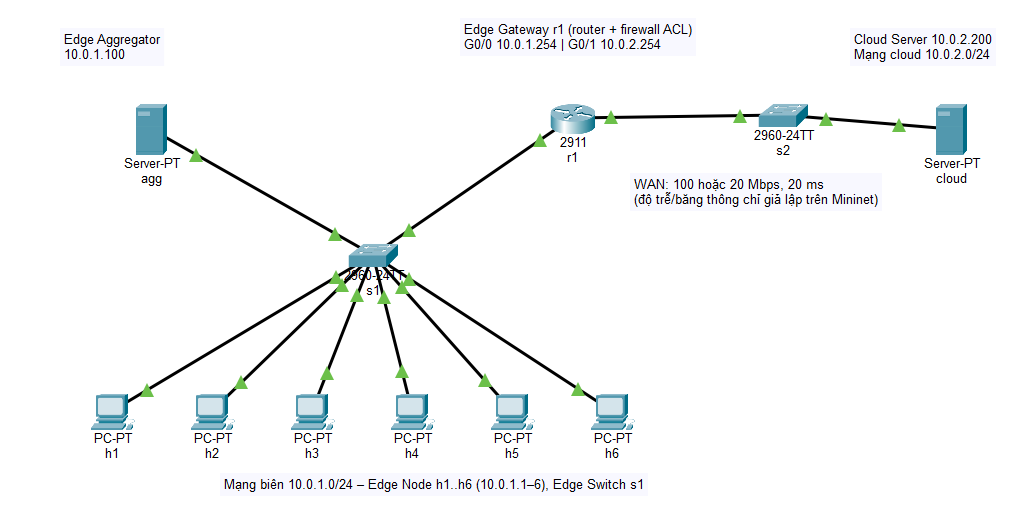
\includegraphics[width=\textwidth]{Images/pt/pt_topo.png}
    \caption{Topo Edge--Cloud dựng lại trên Cisco Packet Tracer 9.0.1}
    \label{fig:pt-topo}
\end{figure}

Firewall iptables của \texttt{r1} trên Mininet được thay bằng hai danh sách truy cập mở rộng (extended ACL) áp chiều vào trên hai cổng của router 2911:
\begin{itemize}
    \item \texttt{EDGE\_IN} trên G0/0: cho phép TCP từ 10.0.1.0/24 tới 10.0.2.200 cổng 5000 và ICMP echo, echo-reply; chặn mọi gói còn lại.
    \item \texttt{CLOUD\_IN} trên G0/1: cho phép gói TCP từ cổng 5000 của \texttt{cloud} về mạng biên khi có cờ ACK hoặc RST (từ khoá \texttt{established}, tương ứng luật \texttt{ESTABLISHED} của iptables), cùng ICMP echo, echo-reply; chặn mọi gói còn lại.
\end{itemize}
Khác với conntrack của iptables, \texttt{established} chỉ xét cờ TCP chứ không theo dõi trạng thái kết nối, nên đây là bản tương đương gần đúng.

Kết quả kiểm tra (Hình~\ref{fig:pt-test} và Hình~\ref{fig:pt-acl}):
\begin{itemize}
    \item \texttt{h1} ping \texttt{agg} (cùng mạng) nhận đủ 4/4 gói trả lời. \texttt{h1} ping \texttt{cloud} lần đầu mất 3/4 gói do ARP và cổng switch đang khởi động, các lần sau nhận đủ 4/4 với TTL = 127, tức gói đã đi qua một router.
    \item \texttt{h1} mở \texttt{http://10.0.2.200} (TCP cổng 80) thì trình duyệt báo \emph{Request Timeout}, trong khi \texttt{h2} mở được trang web của \texttt{agg} ở cùng mạng. Cổng 80 bị chặn đúng như firewall chỉ mở cổng 5000.
    \item \texttt{show access-lists} trên \texttt{r1} cho thấy luật \texttt{deny ip any any} của \texttt{EDGE\_IN} khớp 12 gói (các gói SYN HTTP bị chặn và gửi lại), luật cho ICMP echo khớp 10 gói, và luật cho echo-reply của \texttt{CLOUD\_IN} khớp 9 gói.
\end{itemize}

\begin{figure}[H]
    \centering
    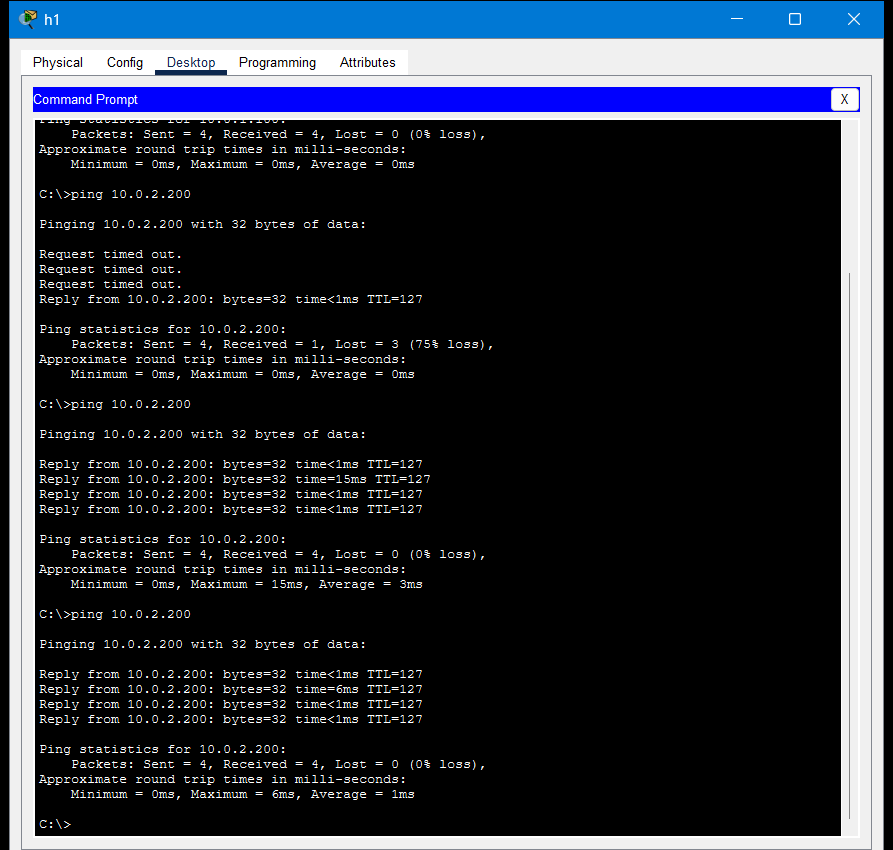
\includegraphics[width=0.62\textwidth]{Images/pt/pt_ping.png}\\[4pt]
    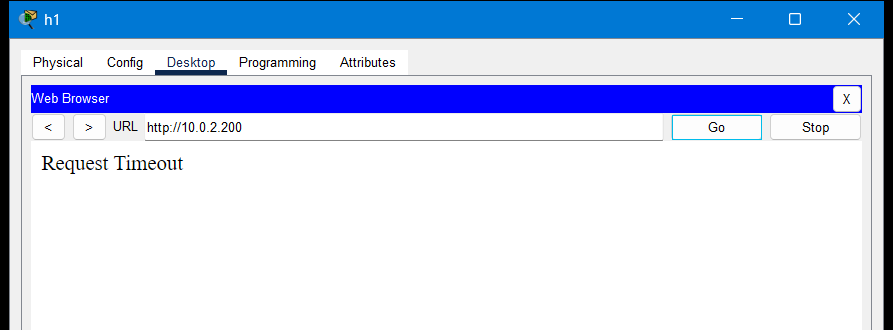
\includegraphics[width=0.62\textwidth]{Images/pt/pt_http.png}
    \caption{Packet Tracer: h1 ping Cloud Server (trên) và truy cập HTTP cổng 80 bị firewall chặn (dưới)}
    \label{fig:pt-test}
\end{figure}

\begin{figure}[H]
    \centering
    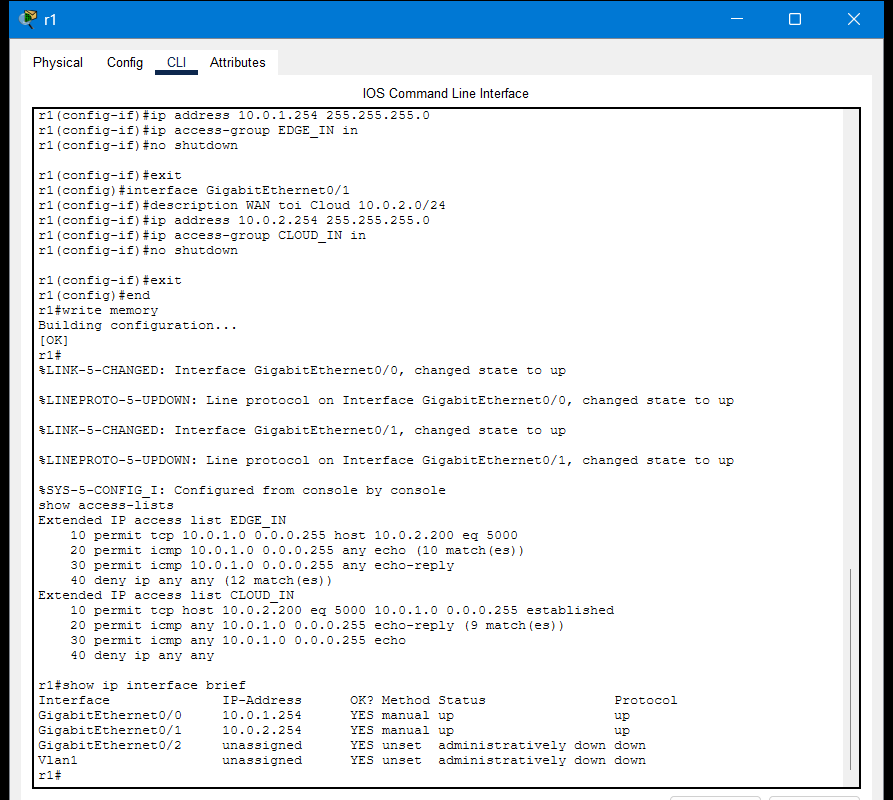
\includegraphics[width=0.75\textwidth]{Images/pt/pt_acl.png}
    \caption{Cấu hình và bộ đếm của ACL trên router r1 trong Packet Tracer}
    \label{fig:pt-acl}
\end{figure}

\subsection{Giao thức ứng dụng FLSync}
FLSync là giao thức tầng ứng dụng do nhóm viết, khoảng 50 dòng Python (\texttt{code/flproto.py}).

\subsubsection{Lý do tự định nghĩa giao thức}
gRPC hay MQTT đều chạy trên TCP và thêm các lớp đóng khung, nén header, quản lý luồng (HTTP/2) hoặc broker trung gian (MQTT). Những lớp này làm khó việc tách riêng hành vi của TCP trên bản bắt gói. Nhóm chọn một giao thức tối giản trên socket TCP để mỗi byte trên đường truyền đều giải thích được.

\subsubsection{Định dạng thông điệp}
Mỗi thông điệp gồm header cố định 20 byte (Bảng~\ref{tab:hdr}) và theo sau là phần payload có độ dài khai báo trong trường \texttt{length}. Payload là các byte 0, vì nội dung không ảnh hưởng tới mạng. Vì TCP là luồng byte không có ranh giới thông điệp, bên nhận đọc đúng 20 byte header trước, sau đó đọc đúng \texttt{length} byte.

\begin{table}[H]
    \centering
    \caption{Header của thông điệp FLSync (big-endian)}
    \label{tab:hdr}
    \begin{tabular}{l c l}
        \toprule
        \textbf{Trường} & \textbf{Byte} & \textbf{Ý nghĩa} \\
        \midrule
        \texttt{magic} & 4 & Chuỗi \texttt{FLSY}, nhận diện giao thức khi xem trên Wireshark \\
        \texttt{version} & 1 & Phiên bản, hiện là 1 \\
        \texttt{type} & 1 & 1 HELLO, 2 GLOBAL, 3 UPDATE, 4 ACK, 5 BYE \\
        \texttt{round} & 4 & Số thứ tự vòng \\
        \texttt{node} & 2 & Định danh Edge Node, 0 là server \\
        \texttt{length} & 8 & Độ dài payload (byte) \\
        \bottomrule
    \end{tabular}
\end{table}

\subsubsection{Trình tự một vòng đồng bộ}
Mỗi Edge Node mở một kết nối TCP duy nhất tới nút tổng hợp và giữ nó qua mọi vòng. Trình tự thông điệp được vẽ trên Hình~\ref{fig:seq}:
\begin{enumerate}
    \item Khởi động: client kết nối, gửi \texttt{HELLO}. Server chờ đủ $N$ client.
    \item Server gửi \texttt{GLOBAL} ($S$ byte) song song cho cả $N$ client, mỗi client một luồng.
    \item Client nhận đủ $S$ byte thì trả về \texttt{ACK} rỗng. Server dùng mốc này để đo $T_{down}$, vì hàm \texttt{sendall()} trả về ngay khi dữ liệu vào bộ đệm gửi của hệ điều hành, trước khi dữ liệu thực sự tới nơi.
    \item Client ngủ 1~s (mô phỏng huấn luyện), rồi gửi \texttt{UPDATE} ($S$ hoặc $S/10$ byte).
    \item Server nhận đủ $N$ bản \texttt{UPDATE}, tổng hợp, gửi \texttt{ACK} kết thúc vòng. $T_{round}$ tính từ lúc bắt đầu gửi \texttt{GLOBAL} tới lúc này.
    \item Sau vòng cuối, server gửi \texttt{BYE} và đóng kết nối (FIN).
\end{enumerate}

\begin{figure}[H]
    \centering
    \begin{tikzpicture}[
        msg/.style={-{Stealth[length=2.5mm]}, thick},
        note/.style={font=\scriptsize, fill=white, inner sep=1pt}
    ]
        \node[font=\small\bfseries] at (0, 0.4) {Edge Node $h_i$};
        \node[font=\small\bfseries] at (8, 0.4) {Aggregator};
        \draw[thick] (0,0) -- (0,-11.2);
        \draw[thick] (8,0) -- (8,-11.2);
        % Bắt tay
        \draw[msg] (0,-0.4) -- node[note, above, sloped] {SYN} (8,-0.9);
        \draw[msg] (8,-1.0) -- node[note, above, sloped] {SYN-ACK} (0,-1.5);
        \draw[msg] (0,-1.6) -- node[note, above, sloped] {ACK + HELLO (20 B)} (8,-2.1);
        \node[font=\scriptsize, anchor=west, align=left] at (8.2,-1.2) {chỉ ở lần\\kết nối đầu};
        % GLOBAL
        \fill[blue!12] (8,-2.6) -- (8,-4.0) -- (0,-4.6) -- (0,-3.2) -- cycle;
        \draw[msg] (8,-2.6) -- (0,-3.2);
        \draw[msg] (8,-4.0) -- (0,-4.6);
        \node[note, fill=blue!12] at (4,-3.6) {GLOBAL: header 20 B + $S$ byte (slow start rồi chia $B/N$)};
        \draw[decorate, decoration={brace, amplitude=4pt}] (8.2,-2.6) -- (8.2,-4.6) node[midway, right=4pt, font=\scriptsize] {$T_{down}$};
        \draw[msg] (0,-4.8) -- node[note, above, sloped] {ACK (FLSync, 20 B)} (8,-5.3);
        % Train
        \draw[fill=gray!20] (-0.25,-5.0) rectangle (0.25,-6.5);
        \node[font=\scriptsize, anchor=east, align=right] at (-0.35,-5.75) {train\\1 s};
        % UPDATE
        \fill[orange!15] (0,-6.6) -- (0,-8.0) -- (8,-8.6) -- (8,-7.2) -- cycle;
        \draw[msg] (0,-6.6) -- (8,-7.2);
        \draw[msg] (0,-8.0) -- (8,-8.6);
        \node[note, fill=orange!15] at (4,-7.6) {UPDATE: 20 B + $S$ (hoặc $S/10$) byte};
        \draw[decorate, decoration={brace, amplitude=4pt}] (8.2,-7.2) -- (8.2,-8.6) node[midway, right=4pt, font=\scriptsize] {$T_{up}$};
        \node[draw, fill=green!10, font=\scriptsize] at (8,-9.1) {FedAvg};
        \draw[msg] (8,-9.6) -- node[note, above, sloped] {ACK (kết thúc vòng $t$)} (0,-10.1);
        \draw[decorate, decoration={brace, amplitude=6pt, mirror}] (9.4,-2.6) -- (9.4,-9.6) node[midway, left=6pt, font=\scriptsize] {$T_{round}$};
        \node[font=\scriptsize] at (4,-10.8) {lặp lại cho vòng $t+1$ trên cùng kết nối TCP};
    \end{tikzpicture}
    \caption{Trình tự thông điệp trong một vòng đồng bộ FLSync}
    \label{fig:seq}
\end{figure}

\subsection{Luồng gói tin qua các tầng}
Hình~\ref{fig:encap} minh hoạ cách một thông điệp \texttt{UPDATE} 10 MB được đóng gói khi đi xuống các tầng tại Edge Node.

\begin{figure}[H]
    \centering
    \begin{tikzpicture}[
        box/.style={draw, minimum height=0.65cm, font=\scriptsize, align=center},
        lay/.style={font=\small\bfseries, anchor=east}
    ]
        \node[lay] at (-0.3, 0) {Application};
        \node[box, fill=yellow!20, minimum width=1.4cm, anchor=west] (a1) at (2.8,0) {FLSync\\20 B};
        \node[box, fill=yellow!8, minimum width=7.0cm, anchor=west] at (a1.east) {payload 10\,000\,000 B (luồng byte, chưa chia gói)};

        \node[lay] at (-0.3, -1.3) {Transport};
        \node[box, fill=red!15, minimum width=1.6cm, anchor=west] (t1) at (2.8,-1.3) {TCP\\20+12 B};
        \node[box, fill=yellow!8, minimum width=3.0cm, anchor=west] (t2) at (t1.east) {đoạn dữ liệu\\1448 B};
        \node[font=\scriptsize, anchor=west] at (t2.east) {\;$\times$ 6907 đoạn};

        \node[lay] at (-0.3, -2.6) {Network};
        \node[box, fill=green!15, minimum width=1.4cm, anchor=west] (n1) at (1.4,-2.6) {IPv4\\20 B};
        \node[box, fill=red!15, minimum width=1.6cm, anchor=west] (n2) at (n1.east) {TCP\\32 B};
        \node[box, fill=yellow!8, minimum width=3.0cm, anchor=west] (n3) at (n2.east) {1448 B};
        \node[font=\scriptsize, anchor=west] at (n3.east) {\;= 1500 B (MTU)};

        \node[lay] at (-0.3, -3.9) {Link};
        \node[box, fill=blue!15, minimum width=1.4cm, anchor=west] (l0) at (0,-3.9) {Ethernet\\14 B};
        \node[box, fill=green!15, minimum width=1.4cm, anchor=west] (l1) at (l0.east) {IPv4\\20 B};
        \node[box, fill=red!15, minimum width=1.6cm, anchor=west] (l2) at (l1.east) {TCP\\32 B};
        \node[box, fill=yellow!8, minimum width=3.0cm, anchor=west] (l3) at (l2.east) {1448 B};
        \node[font=\scriptsize, anchor=west] at (l3.east) {\;= 1514 B / khung};
    \end{tikzpicture}
    \caption{Đóng gói một thông điệp UPDATE qua các tầng}
    \label{fig:encap}
\end{figure}

\subsubsection{Tầng ứng dụng}
FLSync coi mỗi bản mô hình là một thông điệp dài. Ứng dụng gọi \texttt{sendall()} với từng khối 64~KB; hệ điều hành chép dữ liệu vào bộ đệm gửi của socket và trả quyền ngay khi bộ đệm còn chỗ. Ứng dụng không biết dữ liệu đã thực sự tới đích hay chưa, vì vậy giao thức cần thông điệp \texttt{ACK} ở tầng ứng dụng để đo $T_{down}$ chính xác. Tuỳ chọn \texttt{TCP\_NODELAY} được bật để các thông điệp nhỏ (HELLO, ACK) không bị thuật toán Nagle giữ lại.

\subsubsection{Tầng giao vận}
Bắt tay chỉ xảy ra một lần, lúc client kết nối. Gói SYN mang MSS = 1460, Window Scale, SACK Permitted và Timestamps; bắt tay tốn 4~ms với Edge và 44~ms với Cloud. Sau đó TCP chia khối 10 MB thành $\lceil 10^7 / 1448 \rceil = 6907$ đoạn, mỗi đoạn có header 32 byte (20 byte cố định cộng 12 byte Timestamps).

Bên gửi giữ tối đa $\min(cwnd, rwnd)$ byte chưa được xác nhận. Linux tự nới bộ đệm nhận tới 6~MB (giá trị \texttt{tcp\_rmem} mặc định), lớn hơn nhiều so với BDP 550~KB của nhánh WAN. Vì thế $rwnd$ không giới hạn thông lượng trong các kịch bản này; $cwnd$ mới là giới hạn.

Mỗi vòng bắt đầu sau ít nhất 1~s nghỉ. Khoảng nghỉ này dài hơn RTO tối thiểu 200~ms của Linux, nên $cwnd$ bị đặt lại về IW. Theo~\eqref{eq:kstar} của Chương~2, mỗi vòng mất khoảng 2 RTT (8~ms) ở Edge và 6 RTT (264~ms) ở Cloud trước khi lấp đầy link. Theo chiều ngược lại, bên nhận dùng delayed ACK (khoảng 2 đoạn một ACK), tức khoảng 3450 gói ACK 66 byte cho mỗi khối 10 MB.

Khi $N$ kết nối cùng đi qua link \texttt{s1}--\texttt{agg}, hàng đợi 200 gói sẽ có lúc tràn. Gói bị mất làm CUBIC giảm $cwnd$ của luồng đó, và sau vài lần như vậy các luồng về gần mức $B/N$.

\subsubsection{Tầng mạng}
Đường đi ở tầng mạng khác nhau giữa hai kịch bản. Khi tổng hợp tại biên, \texttt{h1} (10.0.1.1) và \texttt{agg} (10.0.1.100) cùng mạng 10.0.1.0/24, nên gói đi thẳng qua \texttt{s1} mà không qua router và TTL giữ nguyên 64.

Khi tổng hợp trên cloud, đích 10.0.2.200 nằm ngoài mạng của \texttt{h1}, nên \texttt{h1} gửi gói tới cổng mặc định 10.0.1.254 (giao diện \texttt{r1-eth0}). Router \texttt{r1} tra bảng định tuyến, thấy 10.0.2.0/24 nối trực tiếp trên \texttt{r1-eth1}, giảm TTL xuống 63, tính lại checksum header IP rồi chuyển gói ra phía WAN. Địa chỉ IP nguồn và đích không đổi vì \texttt{r1} không làm NAT.

Trước khi chuyển, gói phải qua chuỗi FORWARD của iptables trên \texttt{r1}. Chính sách mặc định là DROP. Gói SYN đầu tiên của FLSync khớp luật ``TCP từ 10.0.1.0/24 tới 10.0.2.200 cổng 5000, trạng thái NEW''; module conntrack ghi nhận kết nối, và mọi gói sau đó (cả chiều về) được chấp nhận theo luật ESTABLISHED. Kết nối khác, ví dụ \texttt{h1} thử SSH (TCP/22) tới \texttt{cloud} hoặc \texttt{cloud} chủ động mở kết nối vào mạng biên, bị chặn. Có thể kiểm tra bằng \texttt{h1 nc -zv -w 2 10.0.2.200 22} (phải hết thời gian chờ) và \texttt{r1 iptables -L FORWARD -v} (bộ đếm gói của từng luật).

Cờ DF (cấm phân mảnh) được bật do Linux dùng Path MTU Discovery; mọi link có MTU 1500 nên không có phân mảnh. Trong mạng thật, chặng WAN sẽ đi qua nhiều router; ở đây link \texttt{r1}--\texttt{s2} với 20~ms đại diện cho toàn bộ chặng đó.

\subsubsection{Tầng liên kết}
Trước gói đầu tiên, Edge Node gửi ARP request quảng bá. Với \texttt{agg}, nó hỏi trực tiếp MAC của 10.0.1.100. Với \texttt{cloud}, nó hỏi MAC của cổng mặc định 10.0.1.254, rồi \texttt{r1} tự hỏi MAC của 10.0.2.200 trên mạng cloud. Vì vậy một khung từ \texttt{h1} tới \texttt{cloud} đổi địa chỉ MAC tại router: trên mạng biên, MAC nguồn là của \texttt{h1} và MAC đích là của \texttt{r1-eth0}; trên mạng cloud, MAC nguồn là của \texttt{r1-eth1} và MAC đích là của \texttt{cloud}. Open vSwitch ở chế độ bridge học địa chỉ MAC theo cổng vào và chuyển tiếp khung Ethernet 1514 byte (chưa tính preamble và FCS). Tại cổng ra của link nghẽn, HTB chỉ cho phép 100 Mbit/s đi qua; khung vượt quá nằm chờ trong hàng đợi netem, đây chính là nơi sinh ra $d_{queue}$.

\subsubsection{Chi phí header}
Mỗi đoạn mang 1448 byte dữ liệu trong một khung 1514 byte, hiệu suất:
\begin{equation}
    \eta = \frac{1448}{1514} \approx 0{,}956
    \label{eq:eta}
\end{equation}
Một khối 10 MB vì thế chiếm khoảng $6907 \times 1514 \approx 10{,}46$~MB trên đường truyền (thêm 4{,}6\%), cộng khoảng 0{,}23~MB ACK theo chiều ngược lại. Thông lượng ứng dụng tối đa trên link 100 Mbps là khoảng 95{,}6 Mbps.

\subsection{Kế hoạch bắt gói}
Bắt gói trên giao diện của nút tổng hợp (\texttt{agg-eth0} hoặc \texttt{cloud-eth0}), chỉ lấy 96 byte đầu mỗi gói để file nhỏ:
\codesnap{tcpdump}
Trước khi bắt, tắt các cơ chế offload (TSO, GSO, GRO) trên giao diện bằng \texttt{ethtool}; nếu không, tcpdump sẽ thấy các ``gói'' 64~KB do nhân ghép lại, không thấy được từng đoạn 1448 byte. Script \texttt{run\_experiments.py} đã làm việc này tự động.

Nhóm bắt gói cho hai kịch bản với $N = 4$ và 3 vòng: K1 trên \texttt{agg-eth0}, K3 (WAN 100 Mbps) đồng thời trên \texttt{cloud-eth0}, \texttt{r1-eth0} và \texttt{r1-eth1}. Mỗi file khoảng 31 MB, nằm trong \texttt{results/pcap/}. Do cổng 5000 trùng cổng mặc định của giao thức GSM IPA, Wireshark được mở với tuỳ chọn \texttt{-{}-disable-protocol gsm\_ipa} để phần tải tin hiện đúng là \texttt{Data}. Các ảnh chụp trong báo cáo:
\begin{enumerate}
    \item Bắt tay ba bước và các tuỳ chọn TCP trong gói SYN (Hình~\ref{fig:ws-syn}).
    \item Header FLSync trong khung xem hex: thấy chuỗi \texttt{46 4C 53 59} (``FLSY''), trường \texttt{type} và \texttt{length} (Hình~\ref{fig:ws-hdr}).
    \item Biểu đồ Stevens của luồng \texttt{cloud} $\rightarrow$ \texttt{h1} ở đầu vòng 2, ngay sau khoảng nghỉ huấn luyện (Hình~\ref{fig:ws-stevens}).
    \item I/O Graph của bốn luồng trong kịch bản K1 (Hình~\ref{fig:ws-io}).
    \item Cùng một gói bắt đồng thời trên \texttt{r1-eth1} và \texttt{r1-eth0} (Hình~\ref{fig:ws-router}).
\end{enumerate}

\begin{figure}[H]
    \centering
    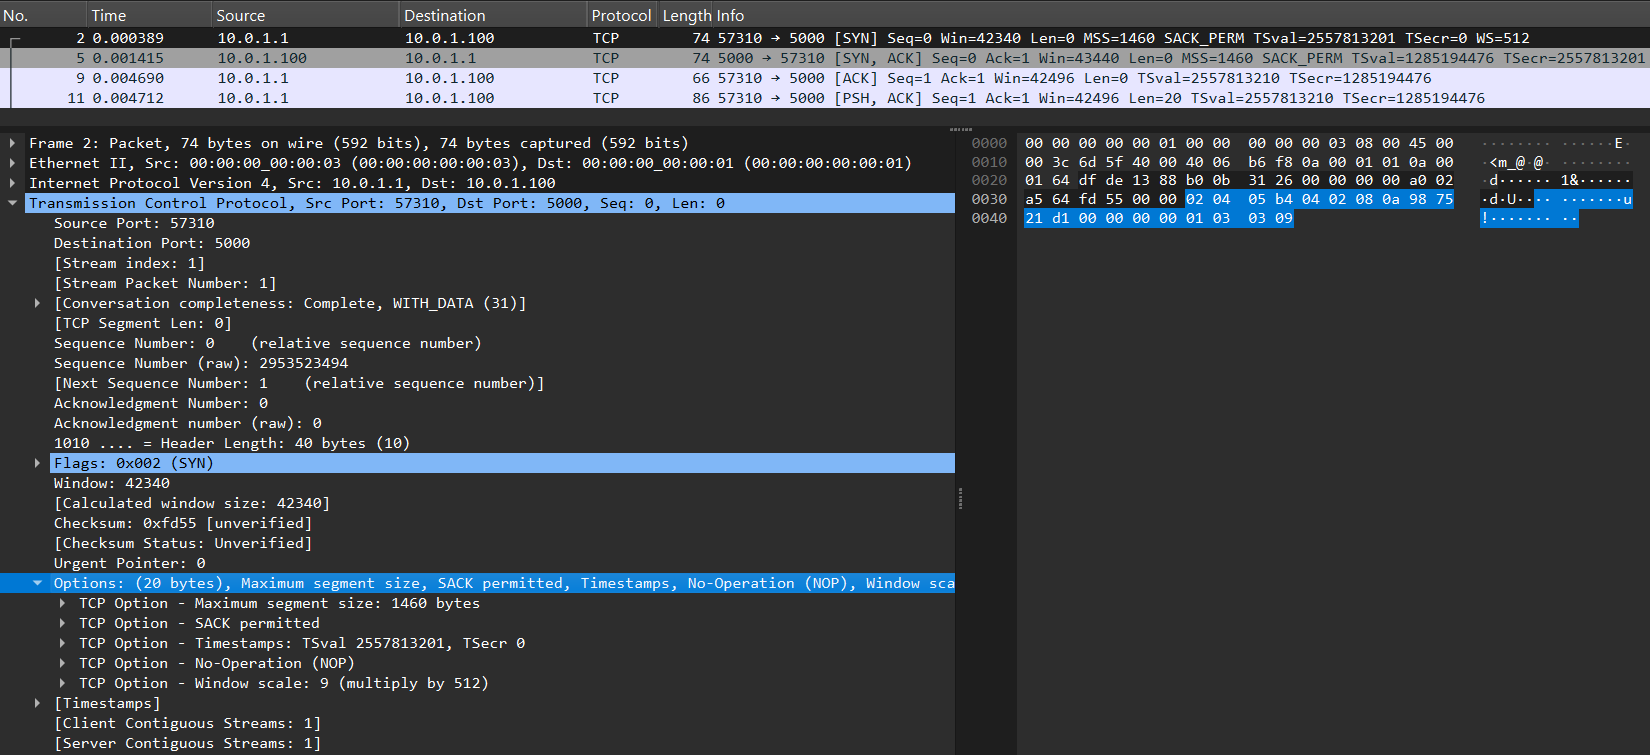
\includegraphics[width=\textwidth]{Images/ws_syn.png}
    \caption{Bắt tay ba bước giữa h1 và Edge Aggregator (K1, gói SYN số 2)}
    \label{fig:ws-syn}
\end{figure}
Gói SYN của \texttt{h1} mang MSS 1460, SACK permitted, Timestamps và Window scale 9 (nhân 512). SYN-ACK của Aggregator được gửi lại sau khoảng 1~ms, với cùng các tuỳ chọn. Gói số 11 là thông điệp HELLO dài 20 byte, gửi ngay sau ACK của bắt tay.

\begin{figure}[H]
    \centering
    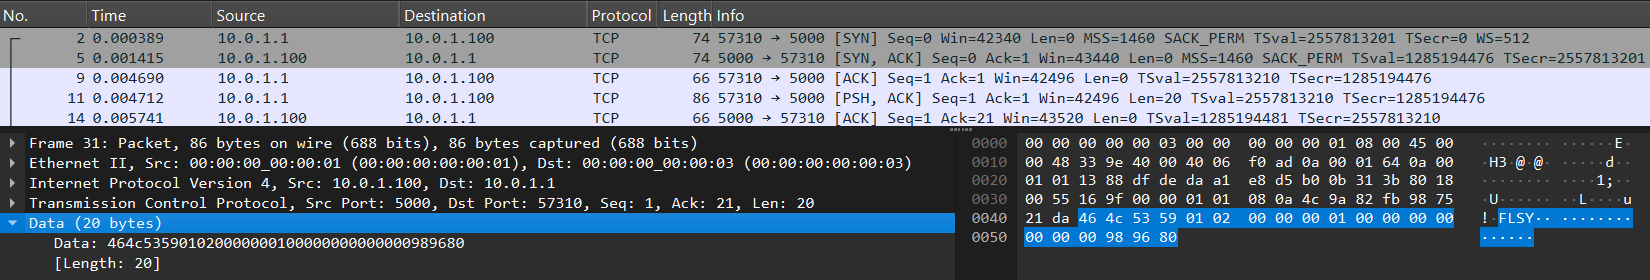
\includegraphics[width=\textwidth]{Images/ws_hdr.png}
    \caption{Header FLSync của thông điệp GLOBAL vòng 1 gửi tới h1 (K1, gói số 31)}
    \label{fig:ws-hdr}
\end{figure}
Vì \texttt{TCP\_NODELAY} được bật và header được gửi bằng một lời gọi \texttt{sendall()} riêng, 20 byte header đi trong một đoạn TCP riêng: \texttt{46 4C 53 59} (magic), \texttt{01} (version), \texttt{02} (GLOBAL), \texttt{00 00 00 01} (vòng 1), \texttt{00 00} (node 0, tức server), \texttt{00 00 00 00 00 98 96 80} (length $= 10\,000\,000$). Các đoạn tải tin sau đó đều dài 1448 byte (19\,472 trên 19\,486 đoạn có dữ liệu trong 30\,000 gói đầu của file).

\begin{figure}[H]
    \centering
    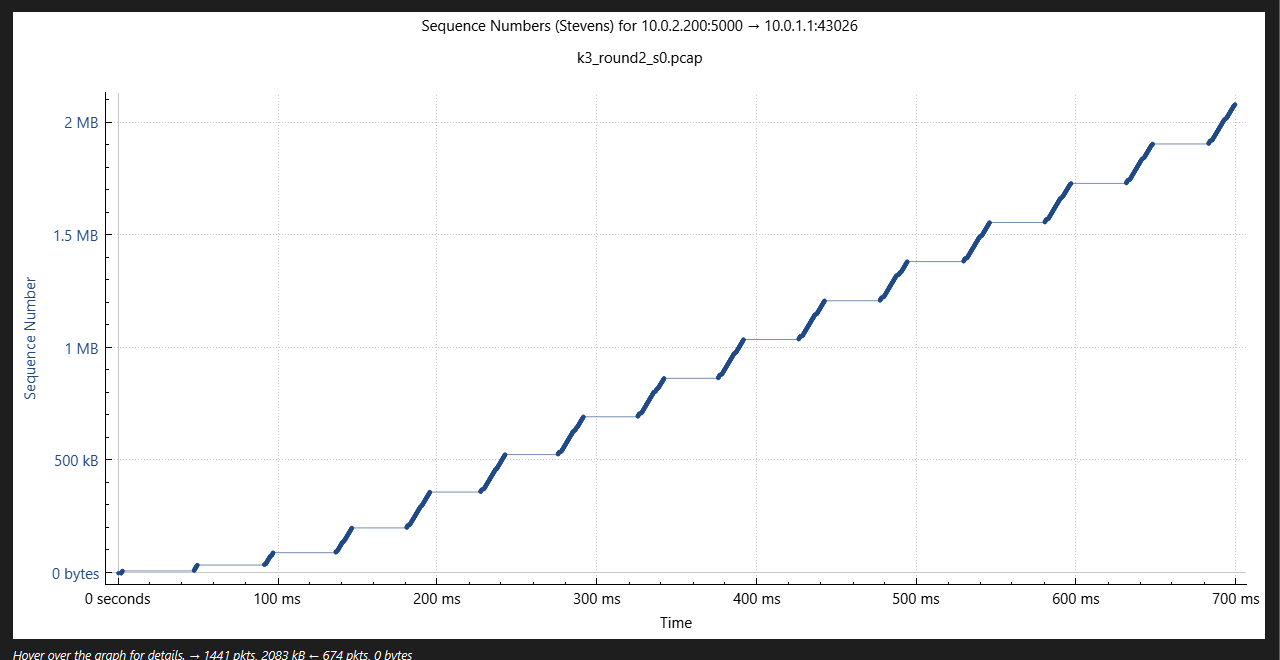
\includegraphics[width=\textwidth]{Images/ws_stevens.png}
    \caption{Biểu đồ Stevens của luồng cloud $\rightarrow$ h1 trong 0{,}7~s đầu vòng 2 (K3, WAN 100 Mbps, $N = 4$)}
    \label{fig:ws-stevens}
\end{figure}

\begin{figure}[H]
    \centering
    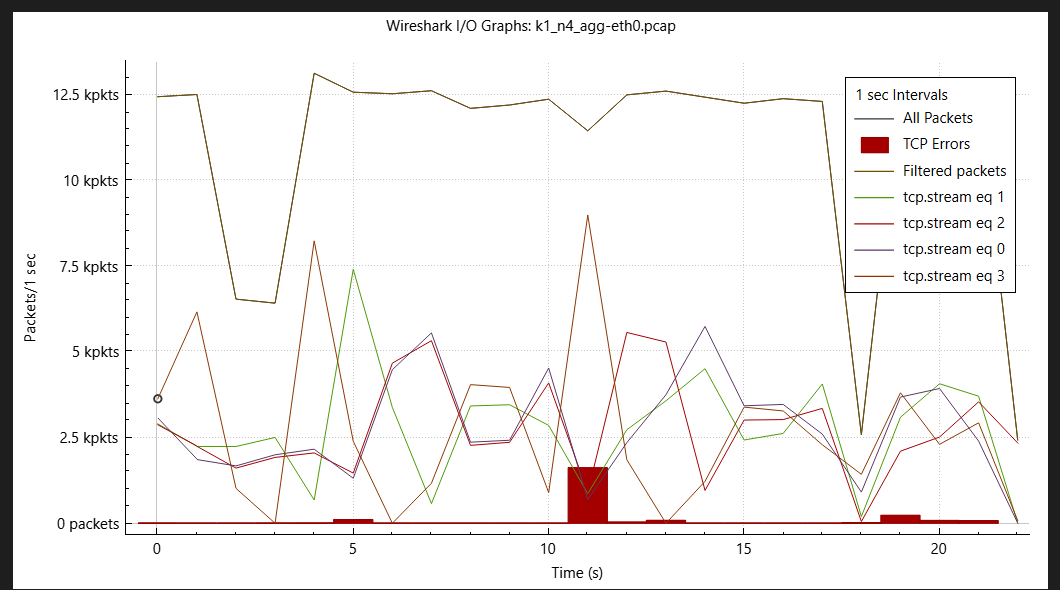
\includegraphics[width=0.9\textwidth]{Images/ws_io.png}
    \caption{I/O Graph của bốn luồng cùng chia link tới Aggregator (K1, $N = 4$, khoảng 1~s)}
    \label{fig:ws-io}
\end{figure}

\begin{figure}[H]
    \centering
    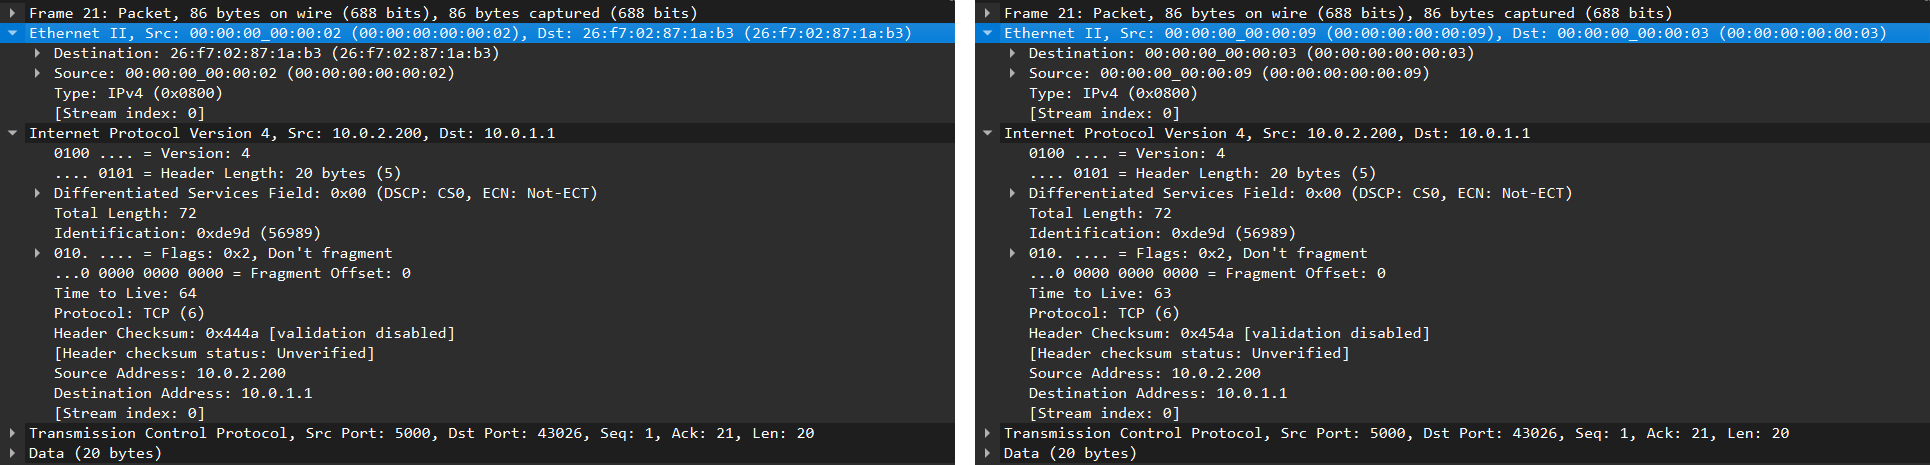
\includegraphics[width=\textwidth]{Images/ws_router.png}
    \caption{Cùng một gói trước (r1-eth1, trái) và sau (r1-eth0, phải) khi đi qua Edge Gateway r1}
    \label{fig:ws-router}
\end{figure}
Hai bản bắt có cùng Identification \texttt{0xde9d}, cùng địa chỉ IP nguồn và đích. Router giảm TTL từ 64 xuống 63, tính lại Header Checksum (\texttt{0x444a} thành \texttt{0x454a}), và thay cả hai địa chỉ MAC: trên mạng cloud khung đi từ \texttt{cloud} (\texttt{00:00:00:00:00:02}) tới \texttt{r1-eth1}; trên mạng biên khung đi từ \texttt{r1-eth0} (\texttt{00:00:00:00:00:09}) tới \texttt{h1} (\texttt{00:00:00:00:00:03}).

\subsection{Kết luận chương}
Topo gồm một nhánh biên RTT 4~ms và một nhánh WAN RTT 44~ms đi qua Edge Gateway \texttt{r1} (router kiêm firewall), cùng băng thông 100 Mbps, cho phép tách riêng ảnh hưởng của RTT. Giao thức FLSync giữ một kết nối TCP mỗi Edge Node, có ACK tầng ứng dụng để đo chính xác từng pha. Header các tầng tốn khoảng 4{,}6\% băng thông. Slow start lặp lại ở mọi vòng vì khoảng nghỉ huấn luyện 1~s dài hơn RTO.

\cleardoublepage
